\documentclass[twoside]{book}

% Packages required by doxygen
\usepackage{calc}
\usepackage{doxygen}
\usepackage{graphicx}
\usepackage[utf8]{inputenc}
\usepackage{makeidx}
\usepackage{multicol}
\usepackage{multirow}
\usepackage{textcomp}
\usepackage[table]{xcolor}

% Font selection
\usepackage[T1]{fontenc}
\usepackage{mathptmx}
\usepackage[scaled=.90]{helvet}
\usepackage{courier}
\usepackage{amssymb}
\usepackage{sectsty}
\renewcommand{\familydefault}{\sfdefault}
\allsectionsfont{%
  \fontseries{bc}\selectfont%
  \color{darkgray}%
}
\renewcommand{\DoxyLabelFont}{%
  \fontseries{bc}\selectfont%
  \color{darkgray}%
}

% Page & text layout
\usepackage{geometry}
\geometry{%
  a4paper,%
  top=2.5cm,%
  bottom=2.5cm,%
  left=2.5cm,%
  right=2.5cm%
}
\tolerance=750
\hfuzz=15pt
\hbadness=750
\setlength{\emergencystretch}{15pt}
\setlength{\parindent}{0cm}
\setlength{\parskip}{0.2cm}
\makeatletter
\renewcommand{\paragraph}{%
  \@startsection{paragraph}{4}{0ex}{-1.0ex}{1.0ex}{%
    \normalfont\normalsize\bfseries\SS@parafont%
  }%
}
\renewcommand{\subparagraph}{%
  \@startsection{subparagraph}{5}{0ex}{-1.0ex}{1.0ex}{%
    \normalfont\normalsize\bfseries\SS@subparafont%
  }%
}
\makeatother

% Headers & footers
\usepackage{fancyhdr}
\pagestyle{fancyplain}
\fancyhead[LE]{\fancyplain{}{\bfseries\thepage}}
\fancyhead[CE]{\fancyplain{}{}}
\fancyhead[RE]{\fancyplain{}{\bfseries\leftmark}}
\fancyhead[LO]{\fancyplain{}{\bfseries\rightmark}}
\fancyhead[CO]{\fancyplain{}{}}
\fancyhead[RO]{\fancyplain{}{\bfseries\thepage}}
\fancyfoot[LE]{\fancyplain{}{}}
\fancyfoot[CE]{\fancyplain{}{}}
\fancyfoot[RE]{\fancyplain{}{\bfseries\scriptsize Generated on Tue Feb 19 2019 22\-:24\-:37 for Aspen by Doxygen }}
\fancyfoot[LO]{\fancyplain{}{\bfseries\scriptsize Generated on Tue Feb 19 2019 22\-:24\-:37 for Aspen by Doxygen }}
\fancyfoot[CO]{\fancyplain{}{}}
\fancyfoot[RO]{\fancyplain{}{}}
\renewcommand{\footrulewidth}{0.4pt}
\renewcommand{\chaptermark}[1]{%
  \markboth{#1}{}%
}
\renewcommand{\sectionmark}[1]{%
  \markright{\thesection\ #1}%
}

% Indices & bibliography
\usepackage{natbib}
\usepackage[titles]{tocloft}
\setcounter{tocdepth}{3}
\setcounter{secnumdepth}{5}
\makeindex

% Hyperlinks (required, but should be loaded last)
\usepackage{ifpdf}
\ifpdf
  \usepackage[pdftex,pagebackref=true]{hyperref}
\else
  \usepackage[ps2pdf,pagebackref=true]{hyperref}
\fi
\hypersetup{%
  colorlinks=true,%
  linkcolor=blue,%
  citecolor=blue,%
  unicode%
}

% Custom commands
\newcommand{\clearemptydoublepage}{%
  \newpage{\pagestyle{empty}\cleardoublepage}%
}


%===== C O N T E N T S =====

\begin{document}

% Titlepage & ToC
\hypersetup{pageanchor=false}
\pagenumbering{roman}
\begin{titlepage}
\vspace*{7cm}
\begin{center}%
{\Large Aspen }\\
\vspace*{1cm}
{\large Generated by Doxygen 1.8.6}\\
\vspace*{0.5cm}
{\small Tue Feb 19 2019 22:24:37}\\
\end{center}
\end{titlepage}
\clearemptydoublepage
\tableofcontents
\clearemptydoublepage
\pagenumbering{arabic}
\hypersetup{pageanchor=true}

%--- Begin generated contents ---
\chapter{Hierarchical Index}
\section{Class Hierarchy}
This inheritance list is sorted roughly, but not completely, alphabetically\-:\begin{DoxyCompactList}
\item \contentsline{section}{Aspen\-:\-:Input\-:\-:Key}{\pageref{d0/d47/class_aspen_1_1_input_1_1_key}}{}
\item \contentsline{section}{Aspen\-:\-:Log\-:\-:Log}{\pageref{de/d89/class_aspen_1_1_log_1_1_log}}{}
\item \contentsline{section}{Aspen\-:\-:Object\-:\-:Object}{\pageref{dc/df6/class_aspen_1_1_object_1_1_object}}{}
\begin{DoxyCompactList}
\item \contentsline{section}{Aspen\-:\-:Engine\-:\-:Engine}{\pageref{de/d64/class_aspen_1_1_engine_1_1_engine}}{}
\item \contentsline{section}{Aspen\-:\-:Event\-:\-:Event\-Handler}{\pageref{de/da8/class_aspen_1_1_event_1_1_event_handler}}{}
\item \contentsline{section}{Aspen\-:\-:Event\-:\-:Event\-Listener}{\pageref{d0/d1f/class_aspen_1_1_event_1_1_event_listener}}{}
\begin{DoxyCompactList}
\item \contentsline{section}{Aspen\-:\-:Event\-:\-:Key\-Event\-Listener}{\pageref{d3/dd2/class_aspen_1_1_event_1_1_key_event_listener}}{}
\item \contentsline{section}{Aspen\-:\-:Event\-:\-:Quit\-Event\-Listener}{\pageref{d3/d97/class_aspen_1_1_event_1_1_quit_event_listener}}{}
\end{DoxyCompactList}
\item \contentsline{section}{Aspen\-:\-:Graphics\-:\-:Graphics}{\pageref{d3/d06/class_aspen_1_1_graphics_1_1_graphics}}{}
\item \contentsline{section}{Aspen\-:\-:Graphics\-:\-:Sprite}{\pageref{d4/d38/class_aspen_1_1_graphics_1_1_sprite}}{}
\end{DoxyCompactList}
\end{DoxyCompactList}

\chapter{Class Index}
\section{Class List}
Here are the classes, structs, unions and interfaces with brief descriptions\-:\begin{DoxyCompactList}
\item\contentsline{section}{\hyperlink{class_aspen_1_1_engine_1_1_engine}{Aspen\-::\-Engine\-::\-Engine} }{\pageref{de/d64/class_aspen_1_1_engine_1_1_engine}}{}
\item\contentsline{section}{\hyperlink{class_aspen_1_1_event_1_1_event_handler}{Aspen\-::\-Event\-::\-Event\-Handler} }{\pageref{de/da8/class_aspen_1_1_event_1_1_event_handler}}{}
\item\contentsline{section}{\hyperlink{class_aspen_1_1_event_1_1_event_listener}{Aspen\-::\-Event\-::\-Event\-Listener} }{\pageref{d0/d1f/class_aspen_1_1_event_1_1_event_listener}}{}
\item\contentsline{section}{\hyperlink{class_aspen_1_1_graphics_1_1_graphics}{Aspen\-::\-Graphics\-::\-Graphics} }{\pageref{d3/d06/class_aspen_1_1_graphics_1_1_graphics}}{}
\item\contentsline{section}{\hyperlink{class_aspen_1_1_input_1_1_key}{Aspen\-::\-Input\-::\-Key} }{\pageref{d0/d47/class_aspen_1_1_input_1_1_key}}{}
\item\contentsline{section}{\hyperlink{class_aspen_1_1_event_1_1_key_event_listener}{Aspen\-::\-Event\-::\-Key\-Event\-Listener} }{\pageref{d3/dd2/class_aspen_1_1_event_1_1_key_event_listener}}{}
\item\contentsline{section}{\hyperlink{class_aspen_1_1_log_1_1_log}{Aspen\-::\-Log\-::\-Log} }{\pageref{de/d89/class_aspen_1_1_log_1_1_log}}{}
\item\contentsline{section}{\hyperlink{class_aspen_1_1_object_1_1_object}{Aspen\-::\-Object\-::\-Object} }{\pageref{dc/df6/class_aspen_1_1_object_1_1_object}}{}
\item\contentsline{section}{\hyperlink{class_aspen_1_1_event_1_1_quit_event_listener}{Aspen\-::\-Event\-::\-Quit\-Event\-Listener} }{\pageref{d3/d97/class_aspen_1_1_event_1_1_quit_event_listener}}{}
\item\contentsline{section}{\hyperlink{class_aspen_1_1_graphics_1_1_sprite}{Aspen\-::\-Graphics\-::\-Sprite} }{\pageref{d4/d38/class_aspen_1_1_graphics_1_1_sprite}}{}
\end{DoxyCompactList}

\chapter{Class Documentation}
\hypertarget{class_aspen_1_1_engine_1_1_engine}{\section{Aspen\-:\-:Engine\-:\-:Engine Class Reference}
\label{class_aspen_1_1_engine_1_1_engine}\index{Aspen\-::\-Engine\-::\-Engine@{Aspen\-::\-Engine\-::\-Engine}}
}
Inheritance diagram for Aspen\-:\-:Engine\-:\-:Engine\-:\begin{figure}[H]
\begin{center}
\leavevmode
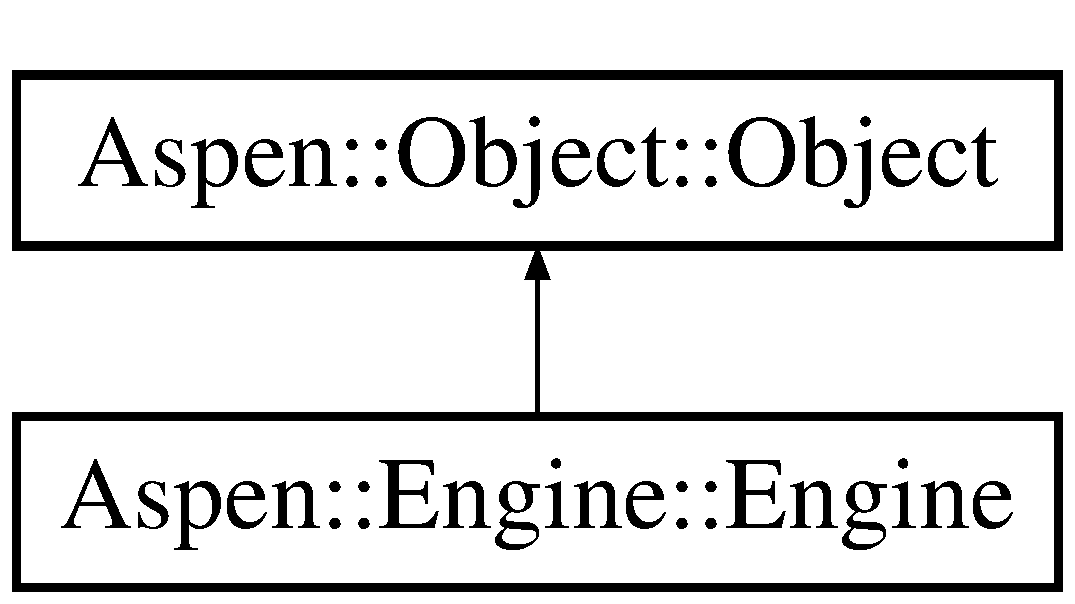
\includegraphics[height=2.000000cm]{de/d64/class_aspen_1_1_engine_1_1_engine}
\end{center}
\end{figure}
\subsection*{Public Member Functions}
\begin{DoxyCompactItemize}
\item 
\hypertarget{class_aspen_1_1_engine_1_1_engine_ac247ab960080cb55b3b3a6202d91259a}{{\bfseries Engine} (int flags=S\-T\-A\-R\-T\-\_\-\-F\-L\-A\-G\-S\-::\-N\-O\-N\-E)}\label{class_aspen_1_1_engine_1_1_engine_ac247ab960080cb55b3b3a6202d91259a}

\item 
\hypertarget{class_aspen_1_1_engine_1_1_engine_afb12d005248a08442a76c2fffd1ad080}{void {\bfseries Refresh\-Graphics} ()}\label{class_aspen_1_1_engine_1_1_engine_afb12d005248a08442a76c2fffd1ad080}

\item 
\hypertarget{class_aspen_1_1_engine_1_1_engine_a14d74ed385c359ecb771843b4af54f21}{\hyperlink{class_aspen_1_1_graphics_1_1_graphics}{Graphics\-::\-Graphics} $\ast$ {\bfseries Graphics} ()}\label{class_aspen_1_1_engine_1_1_engine_a14d74ed385c359ecb771843b4af54f21}

\item 
\hypertarget{class_aspen_1_1_engine_1_1_engine_ad89a5fe88e9424fa67ce36b764dc55b3}{void {\bfseries Refresh\-Event\-Handler} ()}\label{class_aspen_1_1_engine_1_1_engine_ad89a5fe88e9424fa67ce36b764dc55b3}

\item 
\hypertarget{class_aspen_1_1_engine_1_1_engine_a9e5adc83ecc59c18a27da85e4d7b7653}{\hyperlink{class_aspen_1_1_event_1_1_event_handler}{Event\-::\-Event\-Handler} $\ast$ {\bfseries Event\-Handler} ()}\label{class_aspen_1_1_engine_1_1_engine_a9e5adc83ecc59c18a27da85e4d7b7653}

\item 
\hypertarget{class_aspen_1_1_engine_1_1_engine_ab357ce5c8feff1fc480a3db4173ae835}{void {\bfseries Remove\-Child} (Object $\ast$child)}\label{class_aspen_1_1_engine_1_1_engine_ab357ce5c8feff1fc480a3db4173ae835}

\item 
\hypertarget{class_aspen_1_1_engine_1_1_engine_a2a77300f19cece8e61a52ed4cc1526fe}{void {\bfseries Remove\-Child} (int index)}\label{class_aspen_1_1_engine_1_1_engine_a2a77300f19cece8e61a52ed4cc1526fe}

\end{DoxyCompactItemize}
\subsection*{Additional Inherited Members}


The documentation for this class was generated from the following file\-:\begin{DoxyCompactItemize}
\item 
inc/Engine.\-hpp\end{DoxyCompactItemize}

\hypertarget{class_aspen_1_1_event_1_1_event_handler}{\section{Aspen\-:\-:Event\-:\-:Event\-Handler Class Reference}
\label{class_aspen_1_1_event_1_1_event_handler}\index{Aspen\-::\-Event\-::\-Event\-Handler@{Aspen\-::\-Event\-::\-Event\-Handler}}
}
Inheritance diagram for Aspen\-:\-:Event\-:\-:Event\-Handler\-:\begin{figure}[H]
\begin{center}
\leavevmode
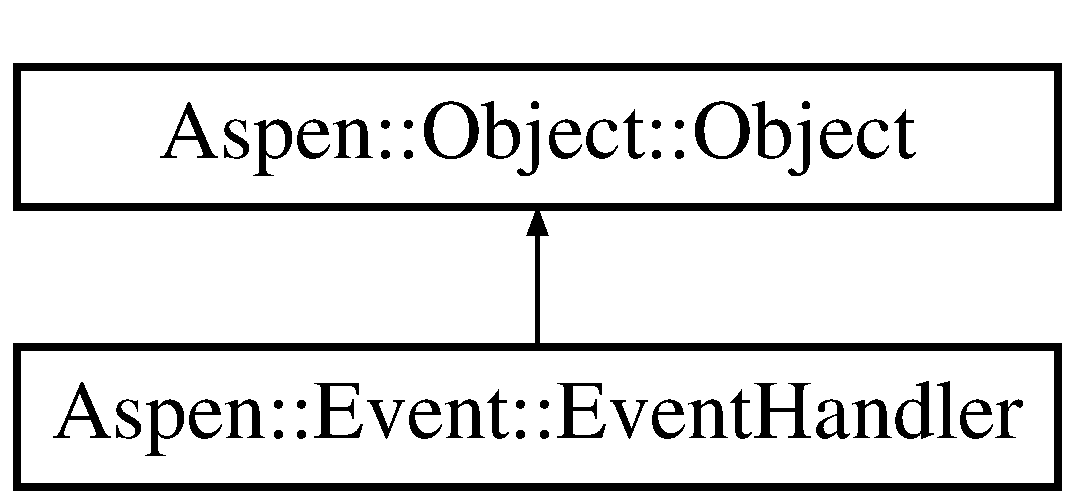
\includegraphics[height=2.000000cm]{de/da8/class_aspen_1_1_event_1_1_event_handler}
\end{center}
\end{figure}
\subsection*{Public Member Functions}
\begin{DoxyCompactItemize}
\item 
\hypertarget{class_aspen_1_1_event_1_1_event_handler_a5d13a2e6bcd952adc6961222627159f7}{void {\bfseries operator()} ()}\label{class_aspen_1_1_event_1_1_event_handler_a5d13a2e6bcd952adc6961222627159f7}

\end{DoxyCompactItemize}
\subsection*{Additional Inherited Members}


The documentation for this class was generated from the following file\-:\begin{DoxyCompactItemize}
\item 
inc/Event.\-hpp\end{DoxyCompactItemize}

\hypertarget{class_aspen_1_1_event_1_1_event_listener}{\section{Aspen\-:\-:Event\-:\-:Event\-Listener Class Reference}
\label{class_aspen_1_1_event_1_1_event_listener}\index{Aspen\-::\-Event\-::\-Event\-Listener@{Aspen\-::\-Event\-::\-Event\-Listener}}
}
Inheritance diagram for Aspen\-:\-:Event\-:\-:Event\-Listener\-:\begin{figure}[H]
\begin{center}
\leavevmode
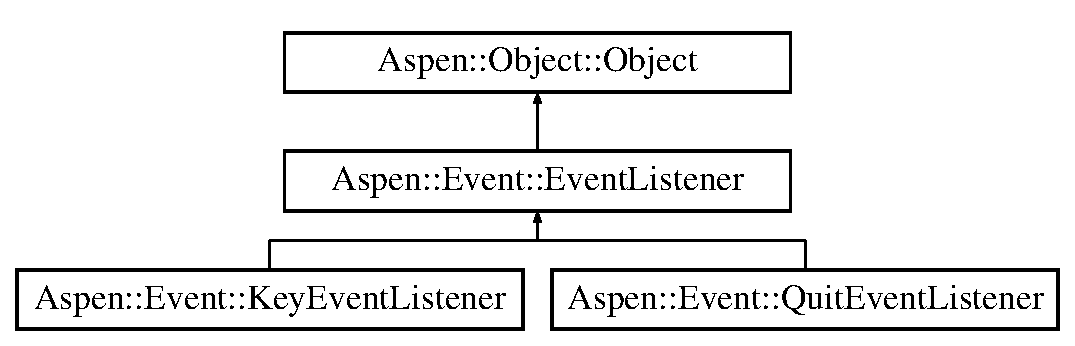
\includegraphics[height=3.000000cm]{d0/d1f/class_aspen_1_1_event_1_1_event_listener}
\end{center}
\end{figure}
\subsection*{Public Member Functions}
\begin{DoxyCompactItemize}
\item 
\hypertarget{class_aspen_1_1_event_1_1_event_listener_a06c80f778a67dbf5216384799f8c9a37}{void {\bfseries operator()} (S\-D\-L\-\_\-\-Event $\ast$event=nullptr)}\label{class_aspen_1_1_event_1_1_event_listener_a06c80f778a67dbf5216384799f8c9a37}

\item 
\hypertarget{class_aspen_1_1_event_1_1_event_listener_ae5c631c56d6086ea145e75c3b2a6da3e}{virtual void {\bfseries Handle} (S\-D\-L\-\_\-\-Event $\ast$event)}\label{class_aspen_1_1_event_1_1_event_listener_ae5c631c56d6086ea145e75c3b2a6da3e}

\end{DoxyCompactItemize}
\subsection*{Additional Inherited Members}


The documentation for this class was generated from the following file\-:\begin{DoxyCompactItemize}
\item 
inc/Event.\-hpp\end{DoxyCompactItemize}

\hypertarget{class_aspen_1_1_graphics_1_1_graphics}{\section{Aspen\-:\-:Graphics\-:\-:Graphics Class Reference}
\label{class_aspen_1_1_graphics_1_1_graphics}\index{Aspen\-::\-Graphics\-::\-Graphics@{Aspen\-::\-Graphics\-::\-Graphics}}
}
Inheritance diagram for Aspen\-:\-:Graphics\-:\-:Graphics\-:\begin{figure}[H]
\begin{center}
\leavevmode
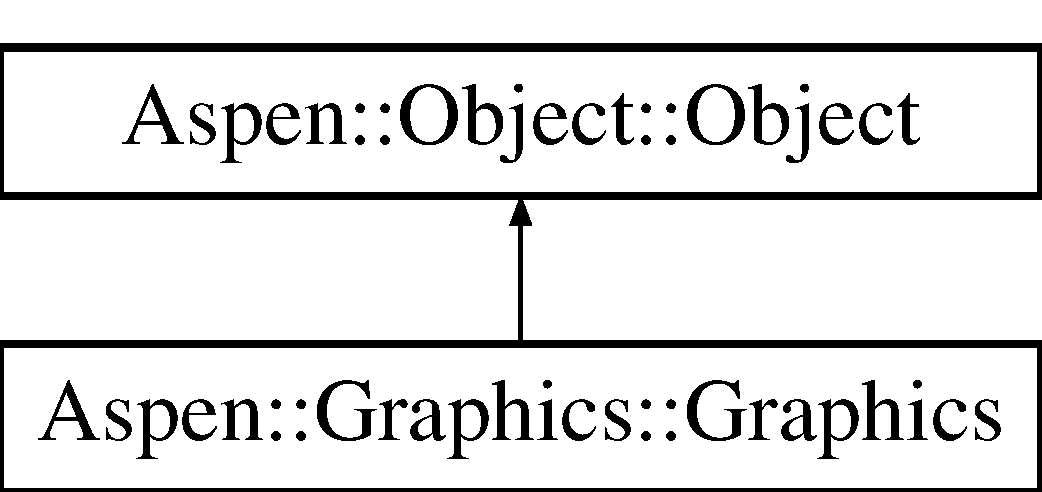
\includegraphics[height=2.000000cm]{d3/d06/class_aspen_1_1_graphics_1_1_graphics}
\end{center}
\end{figure}
\subsection*{Public Member Functions}
\begin{DoxyCompactItemize}
\item 
\hypertarget{class_aspen_1_1_graphics_1_1_graphics_a5a579f9b4a32a45a1647e493d0d7f08a}{{\bfseries Graphics} (int w, int h)}\label{class_aspen_1_1_graphics_1_1_graphics_a5a579f9b4a32a45a1647e493d0d7f08a}

\item 
\hypertarget{class_aspen_1_1_graphics_1_1_graphics_aeb2ae0d78a810c9cebb2271b08a13e89}{void {\bfseries operator()} ()}\label{class_aspen_1_1_graphics_1_1_graphics_aeb2ae0d78a810c9cebb2271b08a13e89}

\item 
\hypertarget{class_aspen_1_1_graphics_1_1_graphics_a7cf3a743431f37d570a7e214f9eccf32}{void {\bfseries Set\-B\-G\-Color} (int r, int g, int b)}\label{class_aspen_1_1_graphics_1_1_graphics_a7cf3a743431f37d570a7e214f9eccf32}

\item 
\hypertarget{class_aspen_1_1_graphics_1_1_graphics_a919a726e4960a1e0cc31264cece8acb7}{S\-D\-L\-\_\-\-Surface $\ast$ {\bfseries Get\-Surface} ()}\label{class_aspen_1_1_graphics_1_1_graphics_a919a726e4960a1e0cc31264cece8acb7}

\item 
\hypertarget{class_aspen_1_1_graphics_1_1_graphics_a8d9158217dd776323ad1073bddd90275}{S\-D\-L\-\_\-\-Window $\ast$ {\bfseries Get\-Window} ()}\label{class_aspen_1_1_graphics_1_1_graphics_a8d9158217dd776323ad1073bddd90275}

\item 
\hypertarget{class_aspen_1_1_graphics_1_1_graphics_adca0e0af6e335deccadc1576a7f4d88a}{void {\bfseries Draw\-Sprite} (\hyperlink{class_aspen_1_1_graphics_1_1_sprite}{Sprite} $\ast$sprite)}\label{class_aspen_1_1_graphics_1_1_graphics_adca0e0af6e335deccadc1576a7f4d88a}

\item 
\hypertarget{class_aspen_1_1_graphics_1_1_graphics_aa1c1efd3d5185a65ce78521064ef5b68}{void {\bfseries End} ()}\label{class_aspen_1_1_graphics_1_1_graphics_aa1c1efd3d5185a65ce78521064ef5b68}

\end{DoxyCompactItemize}
\subsection*{Additional Inherited Members}


The documentation for this class was generated from the following file\-:\begin{DoxyCompactItemize}
\item 
inc/Graphics.\-hpp\end{DoxyCompactItemize}

\hypertarget{class_aspen_1_1_input_1_1_key}{\section{Aspen\-:\-:Input\-:\-:Key Class Reference}
\label{class_aspen_1_1_input_1_1_key}\index{Aspen\-::\-Input\-::\-Key@{Aspen\-::\-Input\-::\-Key}}
}
\subsection*{Public Attributes}
\begin{DoxyCompactItemize}
\item 
\hypertarget{class_aspen_1_1_input_1_1_key_aaa91fee2391f8dbf66eb14e069f2b84b}{bool {\bfseries held}}\label{class_aspen_1_1_input_1_1_key_aaa91fee2391f8dbf66eb14e069f2b84b}

\item 
\hypertarget{class_aspen_1_1_input_1_1_key_a9ff4633c508f52c4f9e966698dbda833}{bool {\bfseries pressed}}\label{class_aspen_1_1_input_1_1_key_a9ff4633c508f52c4f9e966698dbda833}

\item 
\hypertarget{class_aspen_1_1_input_1_1_key_a7e7572c54eb941dac3359c69f35a34d0}{bool {\bfseries released}}\label{class_aspen_1_1_input_1_1_key_a7e7572c54eb941dac3359c69f35a34d0}

\end{DoxyCompactItemize}


The documentation for this class was generated from the following file\-:\begin{DoxyCompactItemize}
\item 
inc/Input.\-hpp\end{DoxyCompactItemize}

\hypertarget{class_aspen_1_1_event_1_1_key_event_listener}{\section{Aspen\-:\-:Event\-:\-:Key\-Event\-Listener Class Reference}
\label{class_aspen_1_1_event_1_1_key_event_listener}\index{Aspen\-::\-Event\-::\-Key\-Event\-Listener@{Aspen\-::\-Event\-::\-Key\-Event\-Listener}}
}
Inheritance diagram for Aspen\-:\-:Event\-:\-:Key\-Event\-Listener\-:\begin{figure}[H]
\begin{center}
\leavevmode
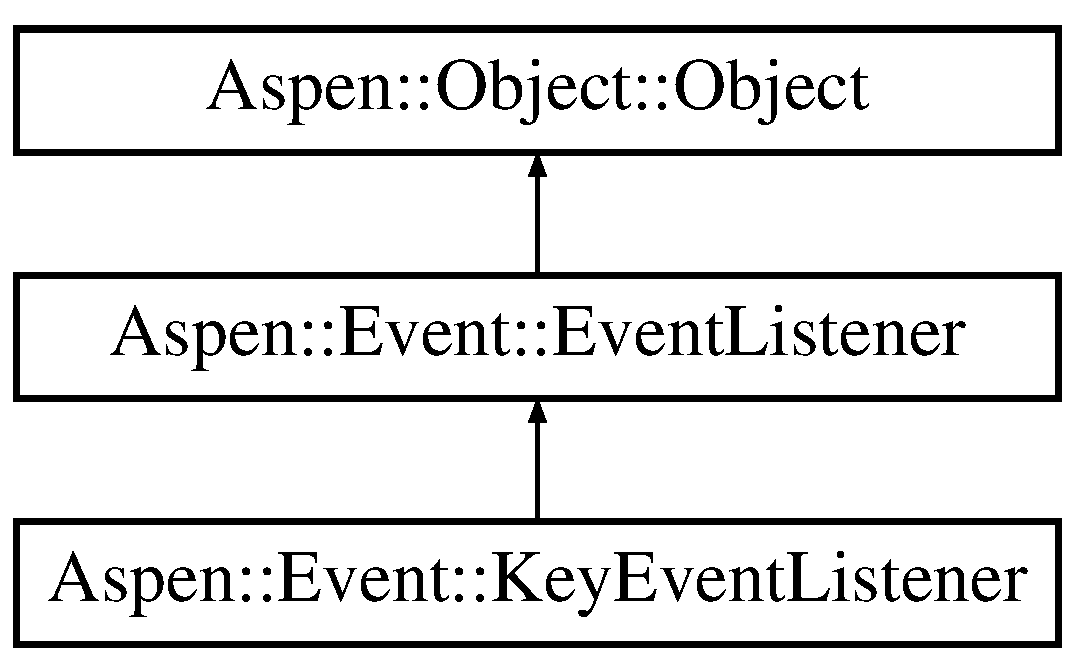
\includegraphics[height=3.000000cm]{d3/dd2/class_aspen_1_1_event_1_1_key_event_listener}
\end{center}
\end{figure}
\subsection*{Public Member Functions}
\begin{DoxyCompactItemize}
\item 
\hypertarget{class_aspen_1_1_event_1_1_key_event_listener_a0affd7ca59069ef53b50cf6af6194c33}{{\bfseries Key\-Event\-Listener} (S\-D\-L\-\_\-\-Keycode k=S\-D\-L\-K\-\_\-\-U\-N\-K\-N\-O\-W\-N)}\label{class_aspen_1_1_event_1_1_key_event_listener_a0affd7ca59069ef53b50cf6af6194c33}

\item 
\hypertarget{class_aspen_1_1_event_1_1_key_event_listener_a76cd7f4e6b5bd314740c419bbd5e2cc7}{void {\bfseries Set\-Key} (S\-D\-L\-\_\-\-Keycode k)}\label{class_aspen_1_1_event_1_1_key_event_listener_a76cd7f4e6b5bd314740c419bbd5e2cc7}

\item 
\hypertarget{class_aspen_1_1_event_1_1_key_event_listener_aea2a17c4e1c8720a18c8c08c21510cad}{void {\bfseries Handle} (S\-D\-L\-\_\-\-Event $\ast$event)}\label{class_aspen_1_1_event_1_1_key_event_listener_aea2a17c4e1c8720a18c8c08c21510cad}

\end{DoxyCompactItemize}
\subsection*{Additional Inherited Members}


The documentation for this class was generated from the following file\-:\begin{DoxyCompactItemize}
\item 
inc/Event.\-hpp\end{DoxyCompactItemize}

\hypertarget{class_aspen_1_1_log_1_1_log}{\section{Aspen\-:\-:Log\-:\-:Log Class Reference}
\label{class_aspen_1_1_log_1_1_log}\index{Aspen\-::\-Log\-::\-Log@{Aspen\-::\-Log\-::\-Log}}
}
\subsection*{Public Member Functions}
\begin{DoxyCompactItemize}
\item 
\hypertarget{class_aspen_1_1_log_1_1_log_a7cd40b18a98f7849ffd0445b1a601634}{{\bfseries Log} (std\-::string prefix=\char`\"{}\char`\"{}, std\-::string suffix=\char`\"{}\char`\"{}, bool print=true)}\label{class_aspen_1_1_log_1_1_log_a7cd40b18a98f7849ffd0445b1a601634}

\item 
\hypertarget{class_aspen_1_1_log_1_1_log_a00c59066f5b3e9385b4ed23d5f75092b}{void {\bfseries operator()} (const std\-::string \&format,...)}\label{class_aspen_1_1_log_1_1_log_a00c59066f5b3e9385b4ed23d5f75092b}

\item 
\hypertarget{class_aspen_1_1_log_1_1_log_a0afd4a9bebc71be10b94a8d910d99336}{void {\bfseries operator()} (const std\-::stringstream \&message)}\label{class_aspen_1_1_log_1_1_log_a0afd4a9bebc71be10b94a8d910d99336}

\item 
\hypertarget{class_aspen_1_1_log_1_1_log_a7aa60eb49286c091b56062c96dc09abf}{void {\bfseries Toggle\-Print} ()}\label{class_aspen_1_1_log_1_1_log_a7aa60eb49286c091b56062c96dc09abf}

\end{DoxyCompactItemize}


The documentation for this class was generated from the following file\-:\begin{DoxyCompactItemize}
\item 
inc/Log.\-hpp\end{DoxyCompactItemize}

\hypertarget{class_aspen_1_1_object_1_1_object}{\section{Aspen\-:\-:Object\-:\-:Object Class Reference}
\label{class_aspen_1_1_object_1_1_object}\index{Aspen\-::\-Object\-::\-Object@{Aspen\-::\-Object\-::\-Object}}
}
Inheritance diagram for Aspen\-:\-:Object\-:\-:Object\-:\begin{figure}[H]
\begin{center}
\leavevmode
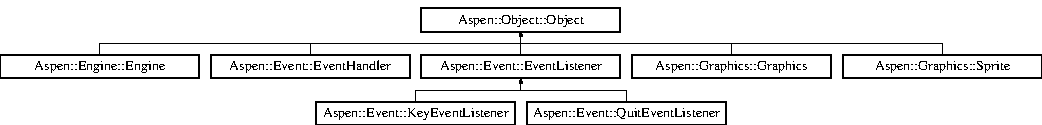
\includegraphics[height=1.680000cm]{dc/df6/class_aspen_1_1_object_1_1_object}
\end{center}
\end{figure}
\subsection*{Public Member Functions}
\begin{DoxyCompactItemize}
\item 
\hypertarget{class_aspen_1_1_object_1_1_object_abba0c3ac64269eb95646b1a07cd3ffae}{{\bfseries Object} (\hyperlink{class_aspen_1_1_object_1_1_object}{Object} $\ast$parent=nullptr)}\label{class_aspen_1_1_object_1_1_object_abba0c3ac64269eb95646b1a07cd3ffae}

\item 
\hypertarget{class_aspen_1_1_object_1_1_object_a8f224e3d221280d5031c7ddf8010eaa0}{\hyperlink{class_aspen_1_1_object_1_1_object}{Object} $\ast$ {\bfseries Parent} ()}\label{class_aspen_1_1_object_1_1_object_a8f224e3d221280d5031c7ddf8010eaa0}

\item 
\hypertarget{class_aspen_1_1_object_1_1_object_a15247881a7c8816de3bdc9099e8cbe65}{\hyperlink{class_aspen_1_1_object_1_1_object}{Object} $\ast$ {\bfseries Root} ()}\label{class_aspen_1_1_object_1_1_object_a15247881a7c8816de3bdc9099e8cbe65}

\item 
\hypertarget{class_aspen_1_1_object_1_1_object_ae827d63a640435d6cf84ef81cd9d1547}{virtual void {\bfseries operator()} ()}\label{class_aspen_1_1_object_1_1_object_ae827d63a640435d6cf84ef81cd9d1547}

\item 
\hypertarget{class_aspen_1_1_object_1_1_object_a512d17c7915076e4e15ca73cfbd67971}{void {\bfseries Add\-Child} (\hyperlink{class_aspen_1_1_object_1_1_object}{Object} $\ast$child)}\label{class_aspen_1_1_object_1_1_object_a512d17c7915076e4e15ca73cfbd67971}

\item 
\hypertarget{class_aspen_1_1_object_1_1_object_ab24f1c4ca5364dc22f4be183c945f437}{{\footnotesize template$<$typename T $>$ }\\T $\ast$ {\bfseries Create\-Child} ()}\label{class_aspen_1_1_object_1_1_object_ab24f1c4ca5364dc22f4be183c945f437}

\item 
\hypertarget{class_aspen_1_1_object_1_1_object_a31d1f3ee496a6247a73d24aac9120c61}{void {\bfseries Remove\-Child} (\hyperlink{class_aspen_1_1_object_1_1_object}{Object} $\ast$child)}\label{class_aspen_1_1_object_1_1_object_a31d1f3ee496a6247a73d24aac9120c61}

\item 
\hypertarget{class_aspen_1_1_object_1_1_object_a22293512e329cc43dd36f2538b2fdcb9}{void {\bfseries Remove\-Child} (int index)}\label{class_aspen_1_1_object_1_1_object_a22293512e329cc43dd36f2538b2fdcb9}

\item 
\hypertarget{class_aspen_1_1_object_1_1_object_a60955e31c71d4171274d28f6f8b38e3c}{\hyperlink{class_aspen_1_1_object_1_1_object}{Object} $\ast$ {\bfseries operator\mbox{[}$\,$\mbox{]}} (int index)}\label{class_aspen_1_1_object_1_1_object_a60955e31c71d4171274d28f6f8b38e3c}

\item 
\hypertarget{class_aspen_1_1_object_1_1_object_a077c6f008bd36517042170c3d589ebfb}{{\footnotesize template$<$typename T $>$ }\\T $\ast$ {\bfseries Find\-Child\-Of\-Type} ()}\label{class_aspen_1_1_object_1_1_object_a077c6f008bd36517042170c3d589ebfb}

\item 
\hypertarget{class_aspen_1_1_object_1_1_object_ac0bd3a26e078850907748692d727230b}{{\footnotesize template$<$typename T $>$ }\\std\-::vector$<$ T $\ast$ $>$ {\bfseries Find\-Children\-Of\-Type} ()}\label{class_aspen_1_1_object_1_1_object_ac0bd3a26e078850907748692d727230b}

\item 
\hypertarget{class_aspen_1_1_object_1_1_object_a2d5e6269408df50277e9377a0ea620de}{const bool \& {\bfseries Valid} () const }\label{class_aspen_1_1_object_1_1_object_a2d5e6269408df50277e9377a0ea620de}

\item 
\hypertarget{class_aspen_1_1_object_1_1_object_a8ca48323f4ac70852f6abdd33042a5b3}{{\bfseries operator bool} () const }\label{class_aspen_1_1_object_1_1_object_a8ca48323f4ac70852f6abdd33042a5b3}

\item 
\hypertarget{class_aspen_1_1_object_1_1_object_a056bfac305482ed281a5d850a2b2754c}{void {\bfseries End} ()}\label{class_aspen_1_1_object_1_1_object_a056bfac305482ed281a5d850a2b2754c}

\end{DoxyCompactItemize}
\subsection*{Protected Member Functions}
\begin{DoxyCompactItemize}
\item 
\hypertarget{class_aspen_1_1_object_1_1_object_aa7b58f0e55a3035f9ab1c958343e5857}{void {\bfseries Set\-Parent} (\hyperlink{class_aspen_1_1_object_1_1_object}{Object} $\ast$parent)}\label{class_aspen_1_1_object_1_1_object_aa7b58f0e55a3035f9ab1c958343e5857}

\end{DoxyCompactItemize}
\subsection*{Protected Attributes}
\begin{DoxyCompactItemize}
\item 
\hypertarget{class_aspen_1_1_object_1_1_object_a3cd9bdc4ee7d3b1ad7ad5a3fcffef228}{\hyperlink{class_aspen_1_1_object_1_1_object}{Object} $\ast$ {\bfseries \-\_\-parent}}\label{class_aspen_1_1_object_1_1_object_a3cd9bdc4ee7d3b1ad7ad5a3fcffef228}

\item 
\hypertarget{class_aspen_1_1_object_1_1_object_a0ad096111db6a0a09fdd5e113d066866}{std\-::vector$<$ \hyperlink{class_aspen_1_1_object_1_1_object}{Object} $\ast$ $>$ {\bfseries \-\_\-children}}\label{class_aspen_1_1_object_1_1_object_a0ad096111db6a0a09fdd5e113d066866}

\item 
\hypertarget{class_aspen_1_1_object_1_1_object_a758956ae85bfe1316609888657092bd5}{bool {\bfseries \-\_\-valid} = false}\label{class_aspen_1_1_object_1_1_object_a758956ae85bfe1316609888657092bd5}

\end{DoxyCompactItemize}
\subsection*{Static Protected Attributes}
\begin{DoxyCompactItemize}
\item 
\hypertarget{class_aspen_1_1_object_1_1_object_a16b58bad3a22150f56ecc37efd19081e}{static int {\bfseries \-\_\-count}}\label{class_aspen_1_1_object_1_1_object_a16b58bad3a22150f56ecc37efd19081e}

\end{DoxyCompactItemize}


The documentation for this class was generated from the following file\-:\begin{DoxyCompactItemize}
\item 
inc/Object.\-hpp\end{DoxyCompactItemize}

\hypertarget{class_aspen_1_1_event_1_1_quit_event_listener}{\section{Aspen\-:\-:Event\-:\-:Quit\-Event\-Listener Class Reference}
\label{class_aspen_1_1_event_1_1_quit_event_listener}\index{Aspen\-::\-Event\-::\-Quit\-Event\-Listener@{Aspen\-::\-Event\-::\-Quit\-Event\-Listener}}
}
Inheritance diagram for Aspen\-:\-:Event\-:\-:Quit\-Event\-Listener\-:\begin{figure}[H]
\begin{center}
\leavevmode
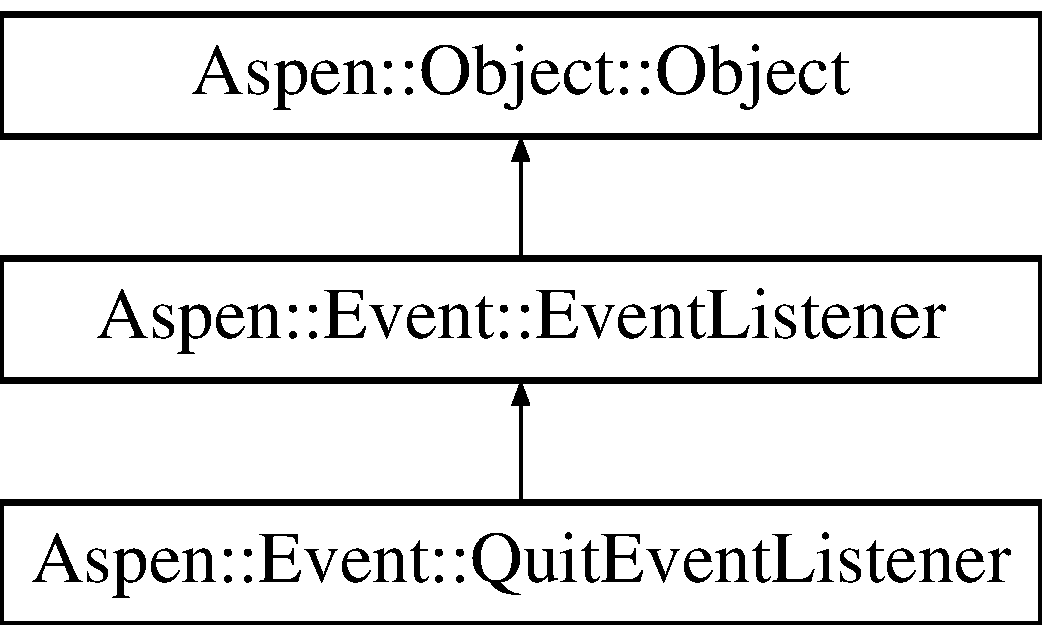
\includegraphics[height=3.000000cm]{d3/d97/class_aspen_1_1_event_1_1_quit_event_listener}
\end{center}
\end{figure}
\subsection*{Public Member Functions}
\begin{DoxyCompactItemize}
\item 
\hypertarget{class_aspen_1_1_event_1_1_quit_event_listener_a58d965225baf29089b4abb738d2c9a57}{void {\bfseries Handle} (S\-D\-L\-\_\-\-Event $\ast$event)}\label{class_aspen_1_1_event_1_1_quit_event_listener_a58d965225baf29089b4abb738d2c9a57}

\end{DoxyCompactItemize}
\subsection*{Additional Inherited Members}


The documentation for this class was generated from the following file\-:\begin{DoxyCompactItemize}
\item 
inc/Event.\-hpp\end{DoxyCompactItemize}

\hypertarget{class_aspen_1_1_graphics_1_1_sprite}{\section{Aspen\-:\-:Graphics\-:\-:Sprite Class Reference}
\label{class_aspen_1_1_graphics_1_1_sprite}\index{Aspen\-::\-Graphics\-::\-Sprite@{Aspen\-::\-Graphics\-::\-Sprite}}
}
Inheritance diagram for Aspen\-:\-:Graphics\-:\-:Sprite\-:\begin{figure}[H]
\begin{center}
\leavevmode
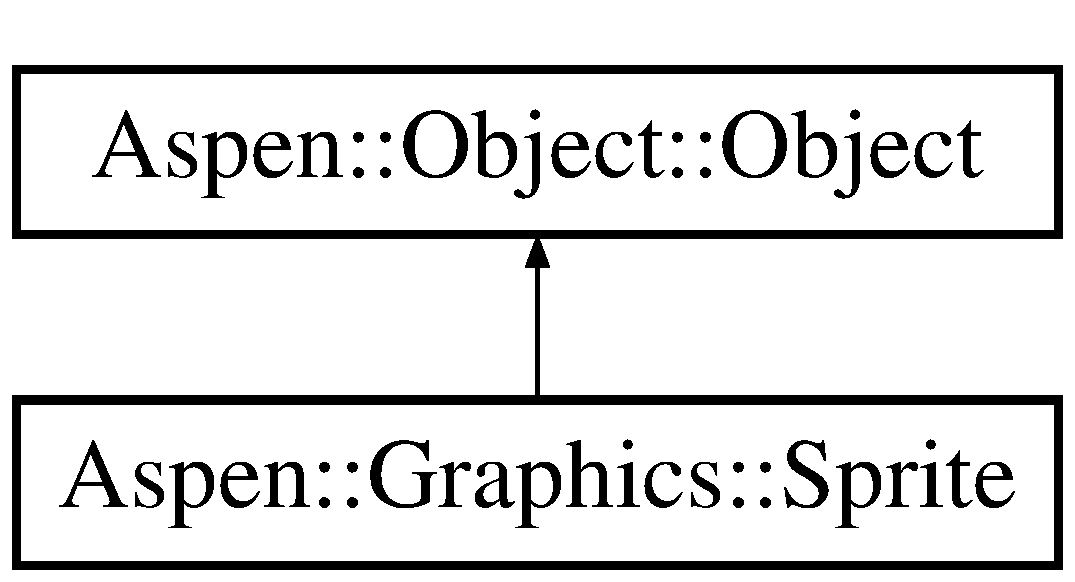
\includegraphics[height=2.000000cm]{d4/d38/class_aspen_1_1_graphics_1_1_sprite}
\end{center}
\end{figure}
\subsection*{Public Member Functions}
\begin{DoxyCompactItemize}
\item 
\hypertarget{class_aspen_1_1_graphics_1_1_sprite_a195d3d73ee898590e80029e2723a2011}{{\bfseries Sprite} (std\-::string path, Object $\ast$parent=nullptr)}\label{class_aspen_1_1_graphics_1_1_sprite_a195d3d73ee898590e80029e2723a2011}

\item 
\hypertarget{class_aspen_1_1_graphics_1_1_sprite_abaa66ca2d23fe08bc9b4941468bf9ebe}{void {\bfseries operator()} ()}\label{class_aspen_1_1_graphics_1_1_sprite_abaa66ca2d23fe08bc9b4941468bf9ebe}

\item 
\hypertarget{class_aspen_1_1_graphics_1_1_sprite_a465f0cab7f12bcf4c4ebc5de59446517}{const std\-::string \& {\bfseries Get\-Path} () const }\label{class_aspen_1_1_graphics_1_1_sprite_a465f0cab7f12bcf4c4ebc5de59446517}

\item 
\hypertarget{class_aspen_1_1_graphics_1_1_sprite_a4e2dbcf2dd4ec0760adb048b0713fa3c}{S\-D\-L\-\_\-\-Surface $\ast$ {\bfseries Get\-Surface} ()}\label{class_aspen_1_1_graphics_1_1_sprite_a4e2dbcf2dd4ec0760adb048b0713fa3c}

\end{DoxyCompactItemize}
\subsection*{Additional Inherited Members}


The documentation for this class was generated from the following file\-:\begin{DoxyCompactItemize}
\item 
inc/Graphics.\-hpp\end{DoxyCompactItemize}

%--- End generated contents ---

% Index
\newpage
\phantomsection
\addcontentsline{toc}{chapter}{Index}
\printindex

\end{document}
